\chapter{}

\titleimg{tcorth}

\mktitle{Capitulum Vicesimum}
\thispagestyle{empty}

\cstart{L}{ocūtusque} est Dominus cūnctōs sermōnēs hōs: 

\vnum{2}``Ego sum Dominus Deus
tuus, quī ēdūxī tē dē terrā Ægyptī, dē domō servitūtis.  \vnum{3}Nōn habēbis deōs
aliēnōs cōram mē. \vnum{4}Nōn faciēs tibi \mpp{sculptile, -is (n):}{rēs secandō facta ut videatur alicuī reī similis, e.g: signum}sculptile, neque omnem
\mpp{similitūdō, -inis (f):}{rēs quae formam aliae reī similem habet; imāgō}similitūdinem quæ est in cælō \mpp{dēsuper:}{ē locō altiore}dēsuper, et
quæ in terrā deorsum, nec eōrum quæ sunt in aquīs sub terrā. 
\vnum{5}Nōn adōrābis
ea, neque cōlēs: ego sum Dominus Deus tuus fortis,
\mpp{zēlōtēs, -ae (m):}{qui amat aliquem et non vult eum aliquem amāre}zēlōtēs, \mpp{vīsitāre:}{vīsum īre}vīsitāns
\mpp{inīquitās, -ātis (f):}{rēs mala ab homine facta; mala anima propter rem malam factam}inīquitātem patrum in fīliōs, in tertiam et quārtam
\mpp{generātio, -ōnis (f):}{e.g una generatio parentibus constat, līberīs
eōrum altera generatio constat, etc...}generātiōnem eōrum quī ōdērunt mē:
\vnum{6}et faciēns \mpp{misericordia, -ae (f):}{quod sentimus dum vidēmus alium
patī}misericordiam in mīllia hīs quī dīligunt mē, et cūstōdiunt
\mpp{praeceptum, -ī:}{quod praecipitur}præcepta mea.''

\vnum{7}``Nōn \mpp{assumere:}{ad mē sumere; aliquem sibi adiungere ad fīnem aliquem capiendum}assūmēs nōmen
Dominī Deī tuī in \mpp{in vānum:}{frūstrā}vānum: nec enim habēbit
\mpp{īnsons, īnsontis (adj):}{quī rem malam nōn fēcit}īnsontem Dominus eum quī assūmpserit nōmen Dominī Deī suī
frūstrā.'' 

\vnum{8}\mpp{mementō:}{memoriā tene}``Mementō ut diem \mpp{sabbatum, -ī (n):}{dies
septimus quō non licet hominibus laborāre}sabbatī
\mpp{sānctificāre:}{sanctum facere}sānctificēs. 
\vnum{9}Sex diēbus operāberis, et
faciēs omnia opera tua. 
\vnum{10}Septimō autem diē sabbatum Dominī Deī tuī est:
nōn faciēs omne opus in eō, tū, et fīlius tuus et fīlia tua, servus tuus et
ancilla tua, \mpp{iūmentum, -ī (n):}{animal utile ad gerendum vel trahendum
e.g, equī, bovēs, et cetera}iūmentum tuum, et advena quī est intrā portās
tuās. 
\vnum{11}Sex enim diēbus fēcit Dominus cælum et terram, et mare, et omnia
quæ in eīs sunt, et requiēvit in diē septimō: \mpp{idcircō:}{proptereā,
ideō}idcircō \mpp{benedīcere:}{sanctum facere}benedīxit Dominus diēī
sabbatī, et sānctificāvit eum.''

\vnum{12}\mpp{honōrāre:}{colere aliquem propter eius virtutēs vel rēs bene factās}``Honōra patrem tuum et
mātrem tuam, ut sīs \mpp{longævus/a/um:}{senex}longævus super terram, quam Dominus
Deus tuus dabit tibi.''

\vnum{13}``Nōn occīdēs.''

\vnum{14}``Nōn \mpp{mœchārī:}{iacēre in lectō cum uxore vel marītō alius}mœchāberis.''

\vnum{15}``Nōn \mpp{fūrtum, -ī (n):}{e.g, si capis pecuniam vel aliquid alius, hoc est furtum}fūrtum faciēs.''

\vnum{16}``Nōn loqueris contrā proximum tuum falsum \mpp{testimōnium, -ī (n):}{id quod ā teste dīcitur}testimōnium.''

\vnum{17}``Nōn \mpp{concupiscere:}{valdē cupere}concupīscēs domum
proximī tuī, nec dēsīderābis uxōrem eius, nōn servum, nōn ancillam, nōn
bovem, nōn asinum, nec omnia quæ illīus sunt.''

\begin{figure}[hp]
    \begin{minipage}[hbp]{0.5\linewidth}
        \centering
        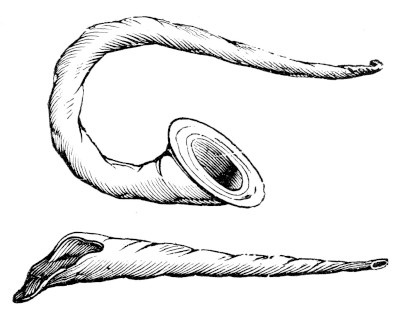
\includegraphics{bucina}
        \caption{buccina, -ae (f)}
    \end{minipage}%
    \begin{minipage}[hbp]{0.5\linewidth}
        \centering
        
\includegraphics{fumus}
        \caption{fūmus, -ī (m)}
    \end{minipage}
\end{figure}

\vnum{18}Cūnctus autem populus
vidēbat vōcēs et \mpp{lampas, lampadis (f):}{ignis}lampadēs, et \mpp{sonitus, -ūs (m):}{sonus
magnus, strepitus}sonitum buccinæ, montemque
\mpp{fūmāre:}{fūmum mittere}fūmantem: et perterritī ac \mpp{pavor, -ōris
(m):}{timor}pavōre \mpp{concussus/a/um:}{pulsātus; turbātus}concussī, stetērunt procul, 
\vnum{19}dīcentēs
Moȳsī: ``Loquere tū nōbīs, et audiēmus: nōn loquātur nōbīs Dominus, nē
forte moriāmur.'' 

\vnum{20}Et ait Moysēs ad populum: ``Nōlīte timēre: ut
enim probāret vōs venit Deus, et ut \mpp{terror, -ōris (m):}{magnus timor}terror illīus
esset in vōbīs, et nōn \mpp{peccātum, -ī:}{res contra legem
acta}peccārētis.''

\vnum{21}Stetitque populus dē longē. Moysēs autem accessit ad
\mpp{cālīgō, cālīginis (f):}{aer per quem difficile est vidēre}cālīginem in quā erat Deus. 

\vnum{22}Dīxit prætereā Dominus ad
Moysēn: ``Hæc dīcēs fīliīs Isrāēl: Vōs
vīdistis quod dē cælō locūtus sim vōbīs. 
\vnum{23}Nōn faciētis deōs argenteōs,
nec deōs aureōs faciētis vōbīs. 
\vnum{24}Altāre dē terrā faciētis mihi, et
offerētis super eō \mpp{holocaustum, -ī (n):}{sacrificium igne factum}holocausta et
\mpp{pācificus/a/um:}{pacem faciens}pācifica vestra, ovēs vestrās et bovēs
in omnī locō in quō memoria fuerit nōminis meī: veniam ad tē, et
\mpp{benedīcere:}{sanctum facere}benedīcam tibi. 
\vnum{25}Quod sī altāre \mimg{rock}{lapis, lapidis (m)}\mpp{lapideus/a/um:}{ex lapidibus factum}lapideum
fēcerīs mihi, nōn ædificābis illud dē sectīs lapidibus: sī
enim levāverīs cultrum super eō, \mpp{polluere:}{foedum facere}polluētur. 
\vnum{26}Nōn ascendēs
per gradūs ad altāre meum, nē \mpp{revēlāre:}{efficere ut aliquid occultum appāreat}revēlētur
\mpp{turpitūdō, -inis (f) <}{turpis}turpitūdō tua.''
